\documentclass[tikz, border=10pt]{standalone}
\usepackage{pgfplots}
\pgfplotsset{compat=1.18}

\begin{document}
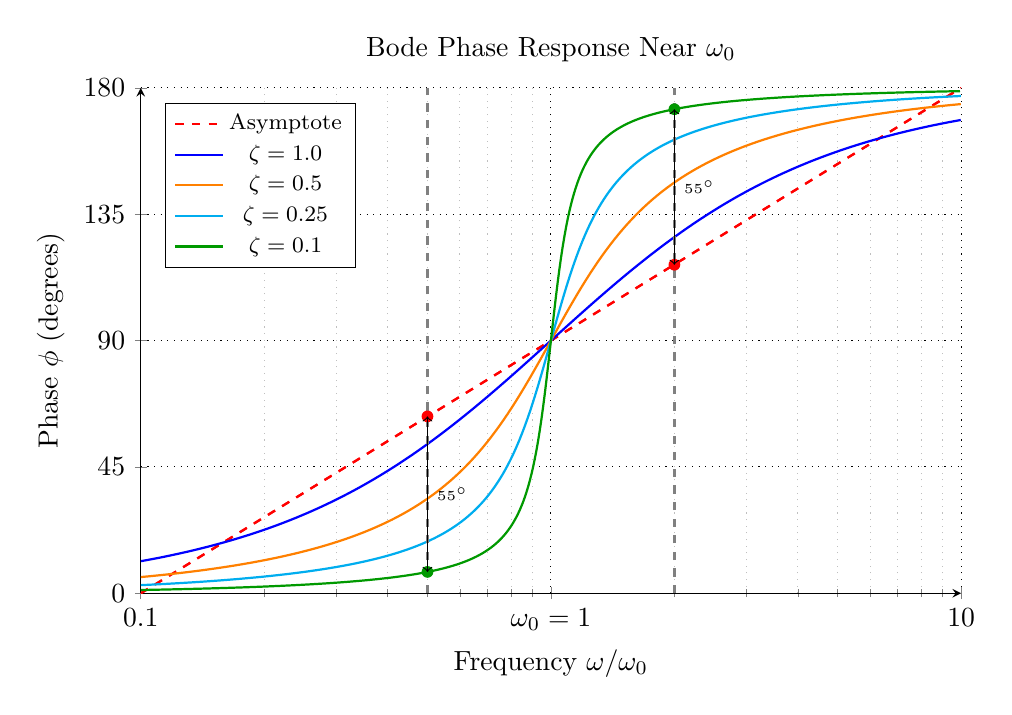
\begin{tikzpicture}
    \begin{semilogxaxis}[
        width=12cm, height=8cm,
        xlabel={Frequency $\omega/\omega_0$},
        ylabel={Phase $\phi$ (degrees)},
        xmin=0.1, xmax=10,
        ymin=0, ymax=180,
        grid=both,
        major grid style={dotted, black},
        minor grid style={dotted, gray!50},
        axis lines=left,
        xtick={0.1, 1, 10},
        xticklabels={$0.1$, $\omega_0=1$, $10$},
        ytick={0, 45, 90, 135, 180},
        legend pos=north west,
        legend style={font=\footnotesize},
        title={Bode Phase Response Near $\omega_0$}
    ]

    % Asymptotes (approximate)
    % 0 for w < 0.1w0
    % 180 for w > 10w0
    % 90 deg/dec slope: y = 90 + 90*log10(x)
    % At x=0.1: 90 - 90 = 0. At x=10: 90 + 90 = 180.
    % We will draw this as a dashed red line.
    \draw[thick, red, dashed] (axis cs: 0.1, 0) -- (axis cs: 0.1, 0) -- (axis cs: 10, 180) -- (axis cs: 10, 180);
    % Wait, straight line from (0.1, 0) to (10, 180) on semilog x
    % This corresponds to linear in log space.
    \addplot[thick, red, dashed, domain=0.1:10] {90 + 90*log10(x)};
    \addlegendentry{Asymptote}

    % Correct Phase: atan2(Im, Re)
    % Re = 1 - x^2. Im = 2*zeta*x.
    % We need phase to go from 0 to 180.
    % atan2 returns angle in (-180, 180]. 
    % Re > 0, Im > 0 -> Q1 (0 to 90)
    % Re < 0, Im > 0 -> Q2 (90 to 180)
    % So standard atan2(Im, Re) works directly if we convert to degrees.

    % Zeta = 1.0 (Double real pole means 2 * atan(x))
    % Correct: The formula is (1 + s/w0)^2 = (1 + jx)^2 = (1-x^2) + j2x.
    % Phase is 2*atan(x).
    \addplot[thick, blue, domain=0.1:10, samples=200] {2*atan(x)};
    \addlegendentry{$\zeta = 1.0$}

    % Zeta = 0.5
    % Phase = atan2(2*zeta*x, 1-x^2)
    % pgfplots 'atan2(y, x)' takes args as (y, x) or (x, y)?
    % PGF manual: atan2(y, x).
    % Note: if 1-x^2 < 0, angle > 90.
    \addplot[thick, orange, domain=0.1:10, samples=200] {atan2(2*0.5*x, 1-x^2)};
    \addlegendentry{$\zeta = 0.5$}
    
    % Zeta = 0.25
    \addplot[thick, cyan, domain=0.1:10, samples=300] {atan2(2*0.25*x, 1-x^2)};
    \addlegendentry{$\zeta = 0.25$}

    % Zeta = 0.1
    \addplot[thick, green!60!black, domain=0.1:10, samples=500] {atan2(2*0.1*x, 1-x^2)};
    \addlegendentry{$\zeta = 0.1$}

    % Correction markers
    \draw[thick, dashed, gray] (axis cs: 0.5, 0) -- (axis cs: 0.5, 180);
    \draw[thick, dashed, gray] (axis cs: 2, 0) -- (axis cs: 2, 180);
    \node[above, gray] at (axis cs: 0.5, 180) {$0.5\omega_0$};
    \node[above, gray] at (axis cs: 2, 180) {$2\omega_0$};

    % Points on asymptote
    \node[circle, fill=red, inner sep=1.5pt] at (axis cs: 0.5, 63) {};
    \node[circle, fill=red, inner sep=1.5pt] at (axis cs: 2, 117) {};

    % Points for zeta=0.1
    \node[circle, fill=green!60!black, inner sep=1.5pt] at (axis cs: 0.5, 7.6) {};
    \node[circle, fill=green!60!black, inner sep=1.5pt] at (axis cs: 2, 172.4) {};

    % Label errors for zeta=0.1
    \draw[<->] (axis cs: 0.5, 7.6) -- (axis cs: 0.5, 63) node[midway, right, font=\tiny] {$55^\circ$};
    \draw[<->] (axis cs: 2, 117) -- (axis cs: 2, 172.4) node[midway, right, font=\tiny] {$55^\circ$};

    \end{semilogxaxis}
\end{tikzpicture}
\end{document}
